% !TEX encoding = UTF-8 Unicode

\documentclass[twocolumn,10pt,a4j]{ltjsarticle}
\usepackage{kougai}

\title{VRコンテンツにおける描写の意図と表現の不一致についての基礎的検討}
\author{2132086 谷 祥英  指導教員 須田 宇宙 准教授}
\date{}

\begin{document}

\maketitle

\section{はじめに}

近年国内のVR市場は拡大しており,立体視と立体音響による知覚の再現と3DCGが主要技術となっている.
仮想空間を現実のように体験できるというVRの特徴から,エンタメや医療,教育など様々な用途で用いられている.
しかし,VR体験中に違和感を生じることが知られている.

ヒトの知覚の約8割は視覚が占めており,VRにおける違和感は視覚的な要因が主因である.
視覚的違和感は機器的な要因とコンテンツ的な要因に大別できる.
機器的な要因について,近年機器性能の向上や身体動作に近い操作法の開発がなされている.

コンテンツ的な要因のひとつに描写の意図と表現の不一致が挙げられる.
これまでに平面視における3DCG映像表現の違和感についての報告などがされているが,立体視における違和感についての報告は少ない.


そこで本研究では,VRコンテンツにおける描写の意図と表現の不一致による違和感について検討する.

%機器的な要因として,dpiやfps,各種トラッキングなどの機器性能による現実の視覚との差や,操作時の空間内と現実との動作の不一致が挙げられる.
%これらは機器性能の向上や身体動作に近い操作法の開発により改善されつつある.
%コンテンツ的な要因として,実写や3DCG,アニメなどの映像表現技法の混用や描写の意図と表現の不一致が挙げられる.
%映像表現技法の混用は,違和感を生じにくい新たな表現技法が登場してきている.
%描写の意図と表現の不一致について,人型の3DCGモデルとそのアニメーションに違和感を感じる例がある.
%立体視は平面視と比較して奥行き知覚や質感を詳細に捉える点で優れ,映像からうける印象は平面視のものと異なることが考えられる.
\section{描写の意図と表現の不一致}
現代ではVRコンテンツ制作が広範化しており,VRコンテンツは実写と3DCGに大別できる.
3DCGによる制作において,個人でも利用できる3DCGモデルやアニメーションは多く多彩な表現が可能な一方で表現次第で違和感を生じることがある.

違和感を生じる例として,現実世界の模倣を意図したコンテンツが挙げられる.
制作者の制作技術や機器の物理演算性能から,細微な動作や現実の物理現象の完全な再現は難しく,キャラクターの表情,服のなびき,動作に違和感が生じることがある.
そのため,%広範の制作者が利用できるリソースでコンテンツ制作する際の,
違和感を生じにくい表現法が望まれる.
関連研究として,平面視における3DCG映像では人体表現,特に頭部の表現が違和感への影響が大きい可能性が報告されている\cite{previous1}.
立体視は平面視と比較し奥行き知覚や質感を詳細に捉える点で優れ,映像からうける印象は平面視のものと異なることが考えられる.

本研究では,リアリティでレベル分けされた人型の3DCGモデルとアニメーションの組み合わせによる印象の如何から違和感について検討していく.

\section{調査概要}
本研究では,刺激映像を呈示し映像のリアリティと違和感の有無について主観評価実験を行った.
呈示刺激は,リアリティの異なる6体の人型の3DCGモデルそれぞれに同一のローデータの歩行動作のアニメーションを適用した映像とした.
映像のリアリティについて,(a)キャラクター的であるか,(b)現実的であるか,(c)人間的であるかをそれぞれ6段階の評価と違和感の有無を調査した.
また違和感の詳細について口述聴取を行った.

各項目の評価の平均と違和感を覚えた被験者の割合を図1,2に示す.
(c)について全映像に共通してどちらかといえば人間的であるという評価が得られた.
(a)の平均が低く(b)の平均が高い映像をリアル指向,(a)の平均が高く(b)の平均が低い映像をデフォルメ指向とすると,映像1,2,3がリアル指向,映像4,5,6がデフォルメ指向であるという評価であった.
リアル指向の映像1,2,3に違和感を覚える割合が比較的高かった.
口述聴取から,機器の描画性能からくるちらつきと,各映像内の現実に即していない頭部や肢体,服装,動作が違和感の要因であった.
デフォルメ指向の映像4に違和感を覚えた割合が最も高く90\%であった.
口述聴取から,モデルの高いデフォルメ度と強い光沢感からくる負感情など,頭部や質感,負感情が違和感の要因であった.
デフォルメ指向の映像5と6に違和感を覚える割合が比較的低く,10\%と50\%であった.
口述聴取から,5では目の大きさ,6では髪型など,頭部が違和感の要因であった.
違和感を覚えなかった理由として,デフォルメ化されたモデルとその質感から,外見と動作が現実に即していなくとも問題がないという回答が多く見受けられた.

%各項目の評価の平均と違和感を覚えた被験者の割合を図1,2に示す.
%(c)について全映像に共通してどちらかといえば人間的であるという評価が得られた.
%デフォルメ指向の映像5と6は,違和感を覚える割合が低く,10\%と50\%であった.
%口述聴取では5について目の大きさ,6について髪型など,頭部に違和感を覚えたという回答が見受けられた.
%違和感を覚えなかった理由として,デフォルメ化されたなモデルとその質感から,外見と動作が現実に即していなくとも問題がないという回答が主であった.
%リアル指向の映像1,2,3は違和感を覚える割合が比較的高かった.
%口述聴取では,頭部や肢体,服装,動作など各モデルの現実に即していない箇所に違和感を覚えていた.また,機器の描画性能によるちらつきを違和感に覚えたという回答も見受けられた.
%デフォルメ指向の映像4は,違和感を覚えた割合が最も高く90\%であった.
%口述聴取では頭部や質感,負感情についての回答が多く,モデルの高いデフォルメ度と強い光沢感からくる負感情が違和感を覚えた要因となっていた.

\begin{figure}[h]
  \centering
  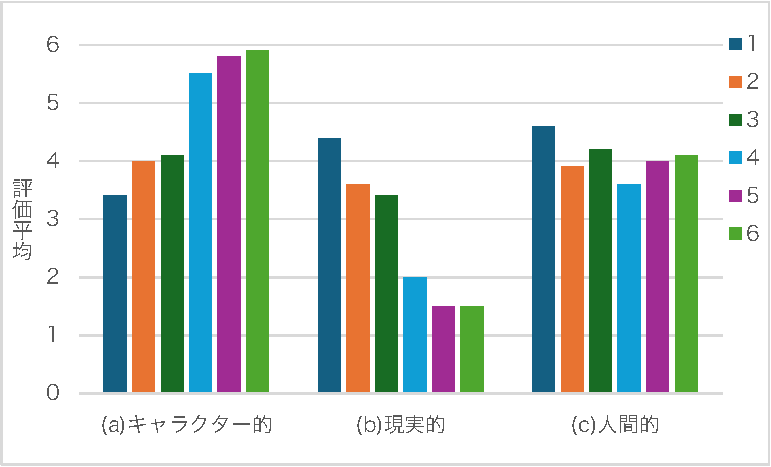
\includegraphics[width=7cm]{fig1.pdf}
  \caption{本実験評価平均}
  \label{fig1}
\end{figure}

\begin{figure}[h]
  \centering
  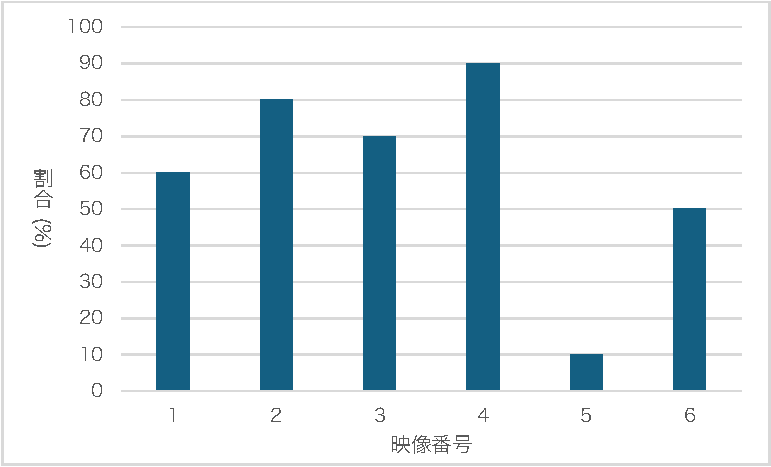
\includegraphics[width=7cm]{fig2.pdf}
  \caption{違和感を覚えた被験者の割合}
  \label{fig1}
\end{figure}


\section{終わりに}
本研究では,人型の3DCGモデルを用いた立体映像の主観評価実験から,VRコンテンツにおける描写の意図と表現の不一致による違和感について調査した.
結果,デフォルメ指向のモデルの使用時に頭部や質感が,リアル指向のモデルの使用時に頭部や肢体,服装,質感,動作,印象が違和感に影響していることが分かった.
今回の実験から得られた違和感を生じた各要素についての対照実験から,違和感への影響について有意性を判断していく必要があると考えられる.

\begin{thebibliography}{99}
\bibitem{previous1}藤原 直子,若月 大輔 : ``リアルな3DCG映像表現の違和感に関する基礎的検討'', \url{https://tsukuba-tech.repo.nii.ac.jp/records/571}, 2025/1/15参照
\end{thebibliography}

\end{document}
